%%%%%%%% SCIS workshop, ICML 2022 EXAMPLE LATEX SUBMISSION FILE %%%%%%%%%%%%%%%%%

\documentclass[nohyperref]{article}

% Recommended, but optional, packages for figures and better typesetting:
\usepackage{microtype}
\usepackage{graphicx}
\usepackage{subfigure}
\usepackage{booktabs} % for professional tables

% hyperref makes hyperlinks in the resulting PDF.
% If your build breaks (sometimes temporarily if a hyperlink spans a page)
% please comment out the following usepackage line and replace
% \usepackage{icml2022} with \usepackage[nohyperref]{icml2022} above.
\usepackage{hyperref}


% Attempt to make hyperref and algorithmic work together better:
\newcommand{\theHalgorithm}{\arabic{algorithm}}

% Use the following line for the initial blind version submitted for review:
\usepackage{icml2022}

% If accepted, instead use the following line for the camera-ready submission:
% \usepackage[accepted]{icml2022}

% For theorems and such
\usepackage{amsmath}
\usepackage{amssymb}
\usepackage{mathtools}
\usepackage{amsthm}

\usepackage{macros}

% if you use cleveref..
\usepackage[capitalize,noabbrev]{cleveref}

%%%%%%%%%%%%%%%%%%%%%%%%%%%%%%%%
% THEOREMS
%%%%%%%%%%%%%%%%%%%%%%%%%%%%%%%%
% \theoremstyle{plain}
% \newtheorem{theorem}{Theorem}[section]
% \newtheorem{proposition}[theorem]{Proposition}
% \newtheorem{lemma}[theorem]{Lemma}
% \newtheorem{corollary}[theorem]{Corollary}
% \theoremstyle{definition}
% \newtheorem{definition}[theorem]{Definition}
% \newtheorem{assumption}[theorem]{Assumption}
% \theoremstyle{remark}
% \newtheorem{remark}[theorem]{Remark}

% Todonotes is useful during development; simply uncomment the next line
%    and comment out the line below the next line to turn off comments
%\usepackage[disable,textsize=tiny]{todonotes}
\usepackage[textsize=tiny]{todonotes}


% The \icmltitle you define below is probably too long as a header.
% Therefore, a short form for the running title is supplied here:
\icmltitlerunning{Submission and Formatting Instructions for the SCIS workshop, ICML 2022}

\begin{document}

\twocolumn[
\icmltitle{Submission and Formatting Instructions for \\
           the SCIS workshop (ICML 2022)}

% It is OKAY to include author information, even for blind
% submissions: the style file will automatically remove it for you
% unless you've provided the [accepted] option to the icml2022
% package.

% List of affiliations: The first argument should be a (short)
% identifier you will use later to specify author affiliations
% Academic affiliations should list Department, University, City, Region, Country
% Industry affiliations should list Company, City, Region, Country

% You can specify symbols, otherwise they are numbered in order.
% Ideally, you should not use this facility. Affiliations will be numbered
% in order of appearance and this is the preferred way.
\icmlsetsymbol{equal}{*}

\begin{icmlauthorlist}
\icmlauthor{Firstname1 Lastname1}{equal,yyy}
\icmlauthor{Firstname2 Lastname2}{equal,yyy,comp}
\icmlauthor{Firstname3 Lastname3}{comp}
\icmlauthor{Firstname4 Lastname4}{sch}
\icmlauthor{Firstname5 Lastname5}{yyy}
\icmlauthor{Firstname6 Lastname6}{sch,yyy,comp}
\icmlauthor{Firstname7 Lastname7}{comp}
%\icmlauthor{}{sch}
\icmlauthor{Firstname8 Lastname8}{sch}
\icmlauthor{Firstname8 Lastname8}{yyy,comp}
%\icmlauthor{}{sch}
%\icmlauthor{}{sch}
\end{icmlauthorlist}

\icmlaffiliation{yyy}{Department of XXX, University of YYY, Location, Country}
\icmlaffiliation{comp}{Company Name, Location, Country}
\icmlaffiliation{sch}{School of ZZZ, Institute of WWW, Location, Country}

\icmlcorrespondingauthor{Firstname1 Lastname1}{first1.last1@xxx.edu}
\icmlcorrespondingauthor{Firstname2 Lastname2}{first2.last2@www.uk}

% You may provide any keywords that you
% find helpful for describing your paper; these are used to populate
% the "keywords" metadata in the PDF but will not be shown in the document
\icmlkeywords{Machine Learning, ICML}

\vskip 0.3in
]

% this must go after the closing bracket ] following \twocolumn[ ...

% This command actually creates the footnote in the first column
% listing the affiliations and the copyright notice.
% The command takes one argument, which is text to display at the start of the footnote.
% The \icmlEqualContribution command is standard text for equal contribution.
% Remove it (just {}) if you do not need this facility.

%\printAffiliationsAndNotice{}  % leave blank if no need to mention equal contribution
\printAffiliationsAndNotice{\icmlEqualContribution} % otherwise use the standard text.

\begin{abstract}
This document provides a basic paper template and submission guidelines.
Abstracts must be a single paragraph, ideally between 4--6 sentences long.
\end{abstract}

\section{Introduction}

In high-dimensional settings, the information captured by the relatively few
labeled training samples is not sufficient for training estimators with good
predictive performance. Therefore, to select among the set of feasible
solutions, one needs to assume a certain structural bias for the estimator
% However, the learning problem becomes tractable if the ground truth has
% certain structural properties that are known a priori
(e.g.\ sparsity, invariance to rotations, translations etc).
For deep neural networks (DNNs), this inductive bias is implicit and recent work [TODO
cite chizat] has revealed that it favors ``sparse'' solutions, similar to an
$\ell_1$ penalty. Moreover, work by [TODO cite telgarsky etc] has shown that
minimizing an exponential loss (e.g.\ logistic, softmax) on separable data leads
to the solution that maximizes the minimum margin on the training set (we refer
to this as the \emph{min-margin solution}).

In order to better understand the behavior of overparameterized neural networks,
in this paper we study simple linear predictors that mirror the structure that
has been observed for DNNs. In particular, we focus on binary classification
with a linear and sparse ground truth. We study the interpolator that maximizes
the min-$\ell_1$-margin (i.e.\ basis pursuit), since a small $\ell_1$ norm is
known to induce sparsity [TODO cite tibshirani etc].

Despite a large trove of positive results for maximum min-margin interpolation
in high dimensions [TODO cite hastie, guillaume, etc], we find that predictors
obtained with basis pursuit 

despite the many positive results for min-l2 margin interpolation, we find that for l1 the error of the estimator deteriorates as d/n increases (in line with konstantin’s paper)

we find that this increase in error for min l1-margin is due to higher variance (since the bias is well aligned with the structure of the GT)

we propose to reduce the variance with avg l1-margin interpolation and find that
indeed it helps reduce variance in high dimensions; moreover, surprisingly, we
see that it also reduces the bias

finally, we discuss limitations of the avg l1-margin solution in low dimensions




\section{Improving stability via average margin interpolation}

In this section we discuss how in high dimensions, the error of the
min-$\ell_1$-margin solution is not optimal even when the ground truth is
sparse. Our synthetic experiments reveal how this phenomenon is particularly
pronounced in high dimensions and provide insights into its causes.


\subsection{High-dimensional setting}
\label{sec:setting}

We consider training data $\DD=\{(x_i, y_i)\}_{i=1}^{n}$ for a binary
classification problem, with $x\in \RR^d$ and $y\in \{-1, +1\}$. We focus
primarily on high-dimensional settings, i.e.\ $d \gg n$ and assume that the
covariates are drawn from a mixture of two truncated Gaussians, each of them
corresponding to one of the two classes. We assume
that the data is noiseless, and hence, there exists a linear classifier with
vanishing Bayes error. Without loss of generality, we assume the Bayes optimal
classifier to be $\thetastar=e_1=[1, 0, ..., 0] \in \RR^d$. We also present
experiments for a $5$-sparse ground truth.

We are interested in analyzing the estimation error of a classifier $\thetahat$,
which captures how well $\thetahat$ recovers the ground truth:

\begin{align}
\err(\thetahat) = \|\thetahat - \thetastar\|_2^2 
\end{align}

Naturally, good estimation error implies good prediction performance as well.


\subsection{Min-margin interpolation}

Consider the estimator that maximizes the min-$\ell_1$-margin of the training
data:

\begin{align}
  \mm =& \arg\max_{\theta} \min_{(x_i, y_i) \in \DD} y_i\theta^\top x_i \\
  &\st
  \|\theta\|_1 \le 1 \text{ and } y_i\theta^\top x_i > 0, \forall i \in [n]
\end{align}

We note that this estimator coincides with the solution to the hard
$\ell_1$-margin SVM problem:

\begin{align}
  \mm = \arg\min_{\theta} \|\theta\|_1 \st y_i\theta^\top x_i \ge 1, \forall i \in
  [n]
\end{align}

\subsection{The problem with min-margin interpolation}

The work of \citet{konstantin} reveals a problem that min-$\ell_1$-margin
interpolation exhibits in high dimensions.  To showcase this issue, let us
compare it to min-l2-margin interpolation, which, unlike the former, lacks the
inductive bias that is expected to make it easier to recover the sparse ground
truth. Despite not having the appropriate inductive bias, \citet{konstantin}
show that the min-l2-margin solution can actually achieve better estimation
error in high dimensions. 
% In particular, as also observed by [TODO konstantin], in the presence of label
% noise, min-l1-margin interpolation achieves worse performance compared to its
% $\ell_2$ counterpart.  As Figure~\at{TODO} reveals,
This failure of is, in large part, due to an increase in the variance of the
min-$\ell_1$-margin solution, despite having a significantly lower bias.

Next we propose an alternative to maximizing the min-$\ell_1$-margin which is
specifically designed to have lower variance in high dimensions.  Surprisingly,
we see that this alternative interpolator also reduces the bias, leading to
smaller estimation error compared to the min-margin solution, even in the
noiseless case.


\begin{figure*}[t]
  \centering
  \begin{subfigure}[t]{0.24\linewidth}
    \centering
    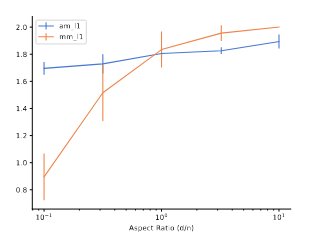
\includegraphics[width=\columnwidth]{figures/estim_err_outlier1.png}
    \label{fig:estim_err_outlier1}
    \caption{}
  \end{subfigure}
  \hfill
  \begin{subfigure}[t]{0.24\linewidth}
    \centering
    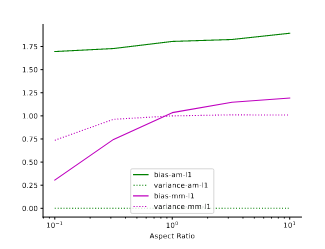
\includegraphics[width=\columnwidth]{figures/bias_variance_outlier1.png}
    \label{fig:bias_variance_outlier1}
    \caption{}
  \end{subfigure}
  \hfill
  \begin{subfigure}[t]{0.24\linewidth}
    \centering
    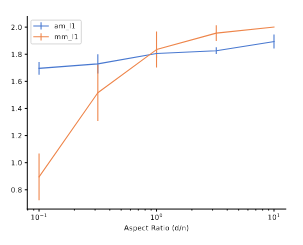
\includegraphics[width=\columnwidth]{figures/estim_err_outlier2.png}
    \label{fig:estim_err_outlier2}
    \caption{}
  \end{subfigure}
  \hfill
  \begin{subfigure}[t]{0.24\linewidth}
    \centering
    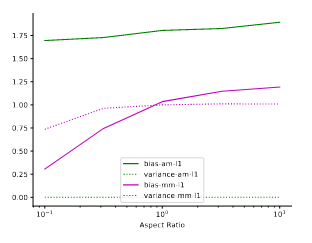
\includegraphics[width=\columnwidth]{figures/bias_variance_outlier2.png}
    \label{fig:bias_variance_outlier2}
    \caption{}
  \end{subfigure}

  \caption{In low dimensions and in the presence of outliers, the average-margin
    solution can have significantly larger estimation error compared to
    min-margin interpolation. Surprisingly, the average-margin classifier is
    more robust in high dimensions (i.e.\ aspect ratio greater than $1$). For
    all experiments we set $d=???$\at{TODO}.} \label{fig:limitations}

\end{figure*}

\subsection{Average-margin interpolation}

In order to reduce the variance of the max-$\ell_1$-margin interpolator, we
propose to study a different interpolating estimator, which maximizes the
\emph{average} $\ell_1$ margin instead of the \emph{minimum} $\ell_1$ margin:

\begin{align}
  \am =& \arg\max_{\theta} \frac{1}{n} \sum_{(x_i, y_i) \in \DD} y_i\theta^\top x_i \\
  &\st
  \|\theta\|_1 \le 1 \text{ and } y_i\theta^\top x_i > 0, \forall i \in [n]
\end{align}

Unlike the min-margin interpolator, the average-margin solution is determined
by \emph{all} the points in the training set. Intuitively, this dependence of
the classifier on all samples is expected to reduce the variance, since it is
less likely that a single point will exert a large influence over the solution
of the optimization problem. This lower variance, combined with the low bias
(which is a consequence of using the $\ell_1$ norm), can decrease the estimation
error compared to min-margin interpolation.


\subsection{Experiments}

We compare average-$\ell_1$-margin and min-$\ell_1$-margin maximization on the
classification problem introduced in Section \at{TODO}. We consider $d=???$ ...
\at{TODO Gizem: describe l1-mm vs l2-mm experiment setting: fixed d, vary n,
how we compute the solutions}. We consider 1-sparse and 5-sparse ground truths.

The main experimental results are illustrated in Figure~\at{TODO}. First, we
notice that the estimation error is significantly reduced by solving the
average-margin optimization problem. Second, the simulations confirm that indeed
the variance of the average-margin solution is much smaller than for the
min-margin interpolator. For a 5-sparse ground truth, the trends remain similar,
with the only mention that the error is slightly larger at the
same $d/n$ ratio. This is expected as the same information (i.e.\ same number of
training samples) is now used to predict more parameters (i.e.\ the $5$
coefficients of the support of $\thetastar$).

In addition, perhaps surprisingly, we notice that avg-margin interpolation also
reduces the bias, which further decreases the error. We leave as future work a
thorough investigation of the mechanism through which average-margin
interpolation leads to lower bias.
% A similar phenomenon has been observed by [TODO our RO paper] where the
% authors note that the 1-sparse ground truth has high average margin, but low
% min margin. 
% Therefore, average-margin maximization is more suitable for recovering
% $\thetastar$.

\subsection{Emergence of average-margin classifiers in practice}

So far we have focused solely on linear models, and hence, a natural question is
whether the insights that we have presented in this section carry over to more
complex classifiers, like deep neural networks.

% Finally, we note that we expect that the insights that we gain using linear
% models carries over to more complex classifiers, like overparameterized deep
% neural networks trained with a suitable loss.
For simplicity, we only study the solution of a convex optimization problem that
we obtain using standard solvers for linear and quadratic programs. However,
prior work allows us to connect the average-margin classifier to certain
predictors that can be achieved in practice.  In particular, \citet{wang21} show
that minimizing a polynomially-tailed loss leads to an estimator akin to the
average-margin solution from Equation~\at{blabla}. Furthermore, \citet{ro}
suggest that conventional regularization techniques like a ridge penalty or
early stopping favor solutions with high average margin (as opposed to the
solution with large min-margin that is found at convergence). In fact, given
that an estimator $\thetahat$ has small norm, writing the Taylor expansion of
the logistic loss leads to precisely the average margin of Equation~\at{bla}.
We leave as future work a thorough analysis of the benefits of maximizing the
average-margin in the context of deep neural networks in the low-sample regime.


\section{Limitations of average-margin interpolation in low dimensions}

Despite its benefits in high dimensions, maximizing the average-margin cannot
replace min-margin interpolation out-of-the-box in any learning problem. In
particular, in low dimensions, when data is plentiful, maximizing the min-margin
turns out to be a more robust option as we illustrate in this section.

Consider the same data distribution as in Section~\at{TODO}, only this time with
the number of samples much larger than the dimensionality $n >> d$. We assume
the data to be noiseless, and hence, interpolation is possible even in this
low-dimensional setting.

Intuitively, average-margin interpolation, just like the mean estimator [TODO
maybe cite bishop or some standard book], is vulnerable to outliers.  To
illustrate this shortcoming, we alter the data distribution by adding a sample
that is far from the true decision boundary for only one of the classes.
If the outlier is far enough, then average-margin interpolation has worse
estimation error than the min-margin solution in low dimensions. Interestingly,
the impact of the outlier on the average-margin interpolator becomes less
significant in high dimensions and $\am$ has once again lower error than $\mm$.


\section{Conclusion and future work}



\bibliography{avg_margin}
\bibliographystyle{icml2022}


%%%%%%%%%%%%%%%%%%%%%%%%%%%%%%%%%%%%%%%%%%%%%%%%%%%%%%%%%%%%%%%%%%%%%%%%%%%%%%%
%%%%%%%%%%%%%%%%%%%%%%%%%%%%%%%%%%%%%%%%%%%%%%%%%%%%%%%%%%%%%%%%%%%%%%%%%%%%%%%
% APPENDIX
%%%%%%%%%%%%%%%%%%%%%%%%%%%%%%%%%%%%%%%%%%%%%%%%%%%%%%%%%%%%%%%%%%%%%%%%%%%%%%%
%%%%%%%%%%%%%%%%%%%%%%%%%%%%%%%%%%%%%%%%%%%%%%%%%%%%%%%%%%%%%%%%%%%%%%%%%%%%%%%
\newpage
\appendix
\onecolumn

\input{appendix}

%%%%%%%%%%%%%%%%%%%%%%%%%%%%%%%%%%%%%%%%%%%%%%%%%%%%%%%%%%%%%%%%%%%%%%%%%%%%%%%
%%%%%%%%%%%%%%%%%%%%%%%%%%%%%%%%%%%%%%%%%%%%%%%%%%%%%%%%%%%%%%%%%%%%%%%%%%%%%%%


\end{document}


% This document was modified from the file originally made available by
% Pat Langley and Andrea Danyluk for ICML-2K. This version was created
% by Iain Murray in 2018, and modified by Alexandre Bouchard in
% 2019 and 2021 and by Csaba Szepesvari, Gang Niu and Sivan Sabato in 2022. 
% Previous contributors include Dan Roy, Lise Getoor and Tobias
% Scheffer, which was slightly modified from the 2010 version by
% Thorsten Joachims & Johannes Fuernkranz, slightly modified from the
% 2009 version by Kiri Wagstaff and Sam Roweis's 2008 version, which is
% slightly modified from Prasad Tadepalli's 2007 version which is a
% lightly changed version of the previous year's version by Andrew
% Moore, which was in turn edited from those of Kristian Kersting and
% Codrina Lauth. Alex Smola contributed to the algorithmic style files.
